% This file was created by matlab2tikz.
%
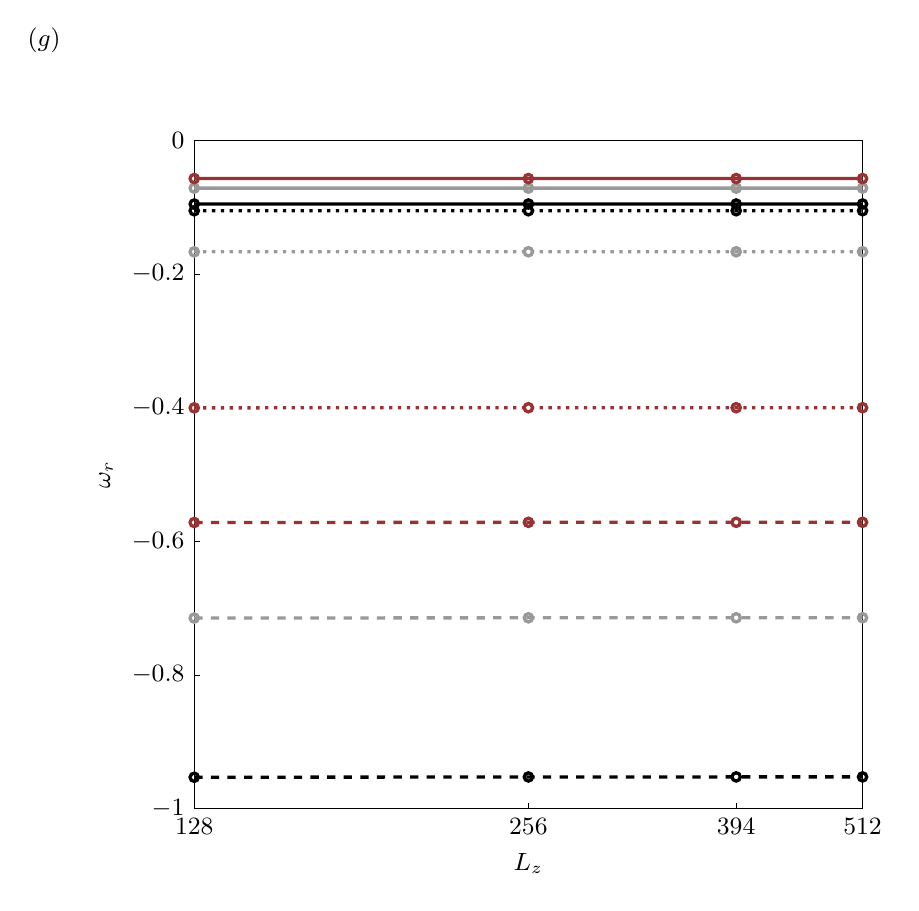
\begin{tikzpicture}

\begin{axis}[%
width=11.255in,
height=7.131in,
at={(1.888in,0.962in)},
scale only axis,
clip=true,
separate axis lines,
every outer x axis line/.append style={black},
every x tick label/.append style={font=\color{black}},
every x tick/.append style={black},
xmode=log,
xmin=128,
xmax=512,
xtick={128,256,394,512},
xticklabels={{128},{256},{394},{512}},
xminorticks=true,
xlabel={$L_z$},
every outer y axis line/.append style={black},
every y tick label/.append style={font=\color{black}},
every y tick/.append style={black},
ymin=-1,
ymax=0,
ylabel={$\omega_r$},
axis background/.style={fill=white},
clip=true,
clip mode=individual,
axis lines=box,
xtick pos=bottom,
ytick pos=left,
tick align=inside,
major tick length=2pt,
width=0.7\linewidth,
height=0.7\linewidth,
every axis/.append style={font=\fontsize{9}{9}\selectfont},xlabel style={font=\fontsize{9}{9}\selectfont},title style={font=\fontsize{9}{9}\selectfont},
legend style={font=\fontsize{8}{9}\selectfont,inner sep=1pt,row sep=1pt,column sep=2pt,nodes={scale=1.00},draw=none},legend image post style={xscale=0.35},
legend columns=1,
scaled x ticks=false,
tick label style={/pgf/number format/fixed,/pgf/number format/precision=2},
every x tick label/.append style={font=\fontsize{9}{9}\selectfont\color{black}},
every y tick label/.append style={font=\fontsize{9}{9}\selectfont\color{black}},
,,
colormap={sigmamap}{rgb(0.0000)=(0.0200,0.1880,0.3800); rgb(0.1000)=(0.0743,0.3456,0.5616); rgb(0.2000)=(0.1918,0.4980,0.7060); rgb(0.3000)=(0.3890,0.6708,0.8226); rgb(0.4000)=(0.7552,0.8682,0.9228); rgb(0.5000)=(0.9690,0.9689,0.9689); rgb(0.6000)=(0.9425,0.8044,0.7614); rgb(0.7000)=(0.8767,0.4910,0.4020); rgb(0.8000)=(0.7869,0.2866,0.2470); rgb(0.9000)=(0.6186,0.1239,0.1568); rgb(1.0000)=(0.4040,0.0000,0.1220)}
]
\addplot [color=black, line width=1.2pt, mark size=1.5pt, mark=o, mark options={solid, black}, forget plot]
  table[row sep=crcr]{%
128	-0.0952982606773163\\
256	-0.0952527810696789\\
394	-0.095244243833798\\
512	-0.0952417234262464\\
};
\addplot [color=black, dashed, line width=1.2pt, mark size=1.5pt, mark=o, mark options={solid, black}, forget plot]
  table[row sep=crcr]{%
128	-0.95296321288197\\
256	-0.952525443979643\\
394	-0.952441794491463\\
512	-0.952416941891964\\
};
\addplot [color=black, dotted, line width=1.2pt, mark size=1.5pt, mark=o, mark options={solid, black}, forget plot]
  table[row sep=crcr]{%
128	-0.10532986633925\\
256	-0.105279414877403\\
394	-0.105269960555207\\
512	-0.105267171099137\\
};
\addplot [color=white!60!black, line width=1.2pt, mark size=1.5pt, mark=o, mark options={solid, white!60!black}, forget plot]
  table[row sep=crcr]{%
128	-0.0714737041396149\\
256	-0.0714395868337803\\
394	-0.0714331831543254\\
512	-0.0714312926960723\\
};
\addplot [color=white!60!black, dashed, line width=1.2pt, mark size=1.5pt, mark=o, mark options={solid, white!60!black}, forget plot]
  table[row sep=crcr]{%
128	-0.714731555359999\\
256	-0.714395203746993\\
394	-0.714331651221535\\
512	-0.714312845169765\\
};
\addplot [color=white!60!black, dotted, line width=1.2pt, mark size=1.5pt, mark=o, mark options={solid, white!60!black}, forget plot]
  table[row sep=crcr]{%
128	-0.166772918384776\\
256	-0.166692482512425\\
394	-0.166677457999391\\
512	-0.166673030172501\\
};
\addplot [color=red!60!teal, line width=1.2pt, mark size=1.5pt, mark=o, mark options={solid, red!60!teal}, forget plot]
  table[row sep=crcr]{%
128	-0.0571790116052954\\
256	-0.0571516752853596\\
394	-0.0571465480992065\\
512	-0.057145034871057\\
};
\addplot [color=red!60!teal, dashed, line width=1.2pt, mark size=1.5pt, mark=o, mark options={solid, red!60!teal}, forget plot]
  table[row sep=crcr]{%
128	-0.571786364240081\\
256	-0.571516299128528\\
394	-0.571465357956675\\
512	-0.571450292917447\\
};
\addplot [color=red!60!teal, dotted, line width=1.2pt, mark size=1.5pt, mark=o, mark options={solid, red!60!teal}, forget plot]
  table[row sep=crcr]{%
128	-0.400255712071431\\
256	-0.400062042724365\\
394	-0.400025922080265\\
512	-0.400015282773083\\
};
\node[right, align=left, inner sep=0]
at (rel axis cs:-0.25,1.15) {$(g)$};
\end{axis}
\end{tikzpicture}%